This chapter describes the method used to design and implement VietFlood. The work followed a software-engineering approach rather than an experimental survey method. First, the main actors and reporting workflow were defined. Second, the report data model was shaped around location, evidence, owner, urgency, severity, and review status. Third, the system was divided into backend services, shared infrastructure utilities, a mobile application, and a web dashboard. Finally, the main workflows were checked through source-level review, local deployment, and end-to-end use of the reporting path. This follows the architectural view that system structure should be guided by responsibilities and quality needs, not only by the chosen technology stack \cite{bass2021softwareArchitecture}.

\section{Requirement Analysis}

The requirement analysis started from the central workflow of the project: a person observes a flood-related situation, submits a report from a mobile device, and an authorized reviewer later inspects the report. VietFlood does not attempt to solve the whole disaster-response process. The method focuses on the part that can be implemented and tested in the prototype: account handling, report submission, evidence upload, report review, and status tracking.

\subsection{Functional Requirements}

The functional requirements were grouped by the three roles supported by the system.

\begin{itemize}
    \item \textbf{Citizen users} can register, sign in, update their profile, create flood reports, provide address and coordinate information, attach photo evidence, and view reports linked to their own account.
    \item \textbf{Relief users} can view broader report lists, open report details, inspect map-related screens, and use report information for field awareness. They do not verify or reject reports in this prototype.
    \item \textbf{Admin users} can use the web dashboard to view all reports, search and filter records, inspect reporter information, preview evidence, update report status, and manage user information.
\end{itemize}

The report object is the center of the system. Each report needs category data, a written description, administrative address fields, coordinates, evidence metadata, a reporter, a severity value, an urgency flag, timestamps, and a review status. The status values are kept simple: \texttt{pending}, \texttt{verified}, \texttt{resolved}, and \texttt{rejected}. This small set is enough for the prototype and avoids a review process that would be too complex for the current scope.

\subsection{Non-Functional Requirements}

The non-functional requirements came from the way the system is expected to be used. The backend should expose one public entry point for mobile and web clients. Authentication and report handling should be separated so identity logic does not become mixed with report storage and evidence handling. Uploaded images should be stored outside the relational database, while report records and evidence metadata remain searchable. The backend should also be deployable through repeatable configuration rather than manual server setup.

These requirements led to four main design decisions. VietFlood uses an API gateway in front of internal services. RabbitMQ carries messages between the gateway, authentication service, and reports service. Cloudinary stores uploaded evidence files, while PostgreSQL stores report records and evidence metadata. Docker Compose is used to run the backend services together with Redis and RabbitMQ in a repeatable environment.

\section{Actor Analysis}

VietFlood has three main actors: citizen, relief, and administrator. The actors were chosen to match the real responsibilities in the prototype. Citizens submit reports, relief users read field information, and administrators review and manage the submitted records.

\subsection{Citizen Actor}

The citizen actor represents a person who notices a flood-related incident and submits the first structured record. The citizen workflow begins with registration or sign-in. After authentication, the user can create a report by selecting a category, writing a description, choosing location information, setting urgency and severity, and attaching optional photos. The mobile app can also help with device location and Vietnam administrative division selection.

\begin{figure}[htbp]
    \centering
    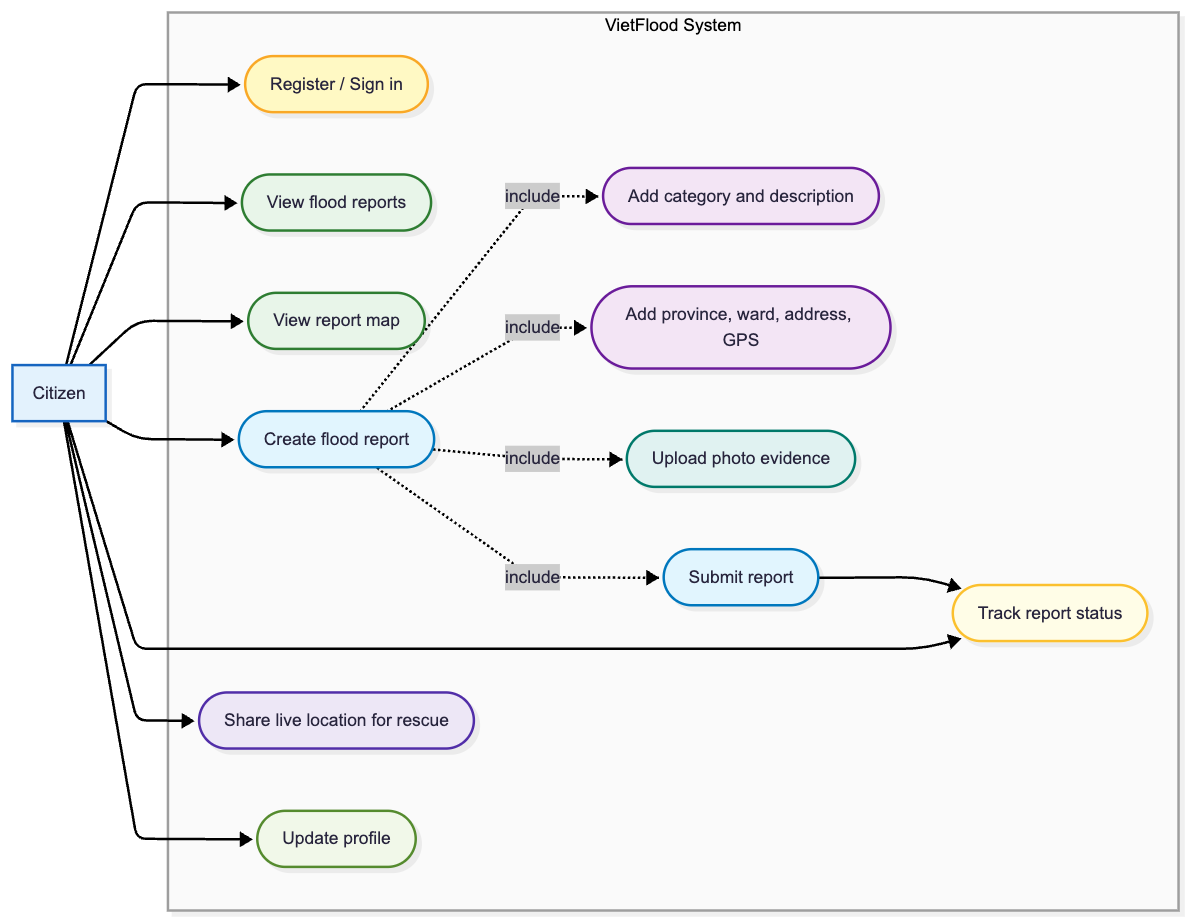
\includegraphics[width=0.74\linewidth,height=0.36\textheight,keepaspectratio]{images/figure3-1-citizen-use-case.png}
    \caption{Use case diagram for the citizen actor in VietFlood.}
    \label{fig:method-citizen-usecase}
\end{figure}

\subsection{Relief Actor}

The relief actor represents users who need situational awareness from the submitted reports. In the mobile app, this role can use report lists, report detail screens, and map-related views. The relief role is deliberately narrower than the admin role. Relief users can inspect information for field awareness, but they do not verify, reject, or administratively close reports in this thesis version.

\begin{figure}[htbp]
    \centering
    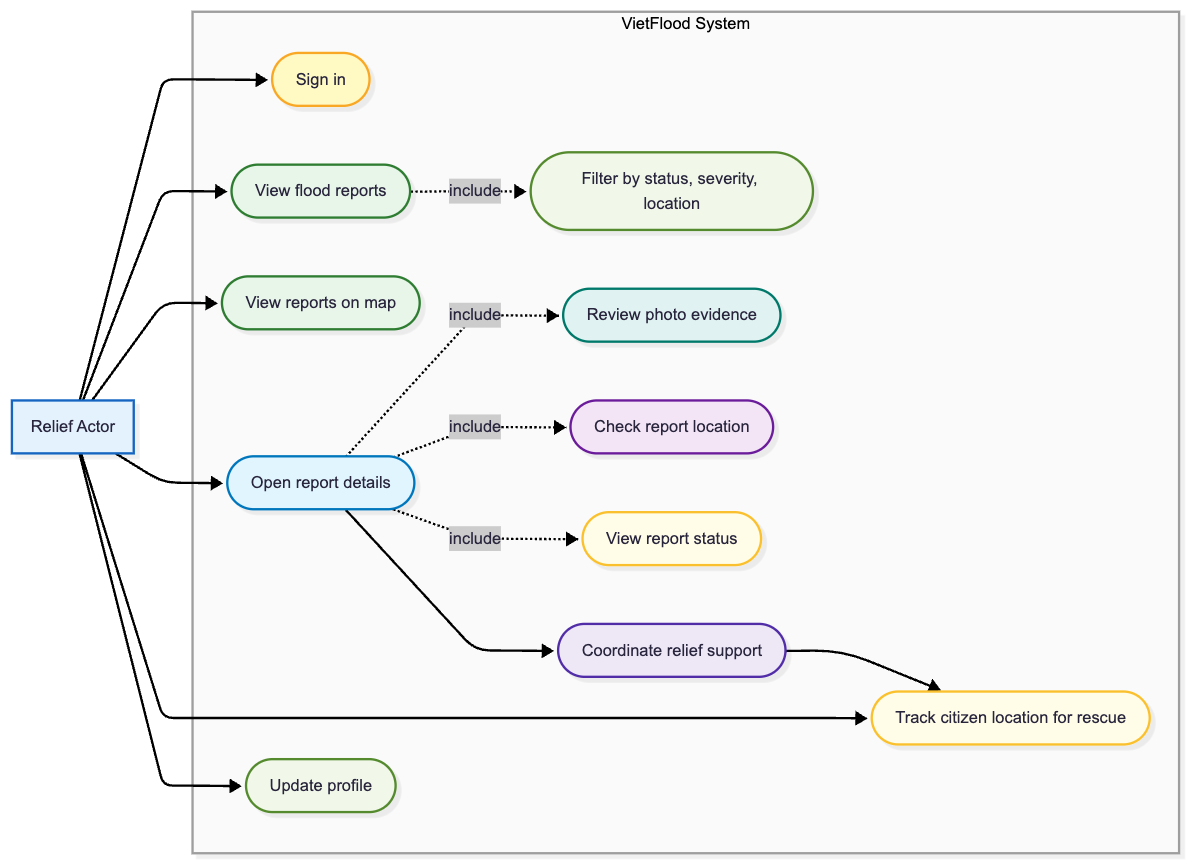
\includegraphics[width=0.74\linewidth,height=0.36\textheight,keepaspectratio]{images/figure3-2-relief-use-case.png}
    \caption{Use case diagram for the relief actor in VietFlood.}
    \label{fig:method-relief-usecase}
\end{figure}

\subsection{Administrator Actor}

The administrator actor works through the web dashboard. The dashboard loads report data through the API gateway and displays report content together with reporter details, status, evidence previews, and filtering controls. Admin users are responsible for changing report status and managing user records. The web client checks the signed-in profile before showing the dashboard so a non-admin account cannot simply open the admin pages.

\begin{figure}[htbp]
    \centering
    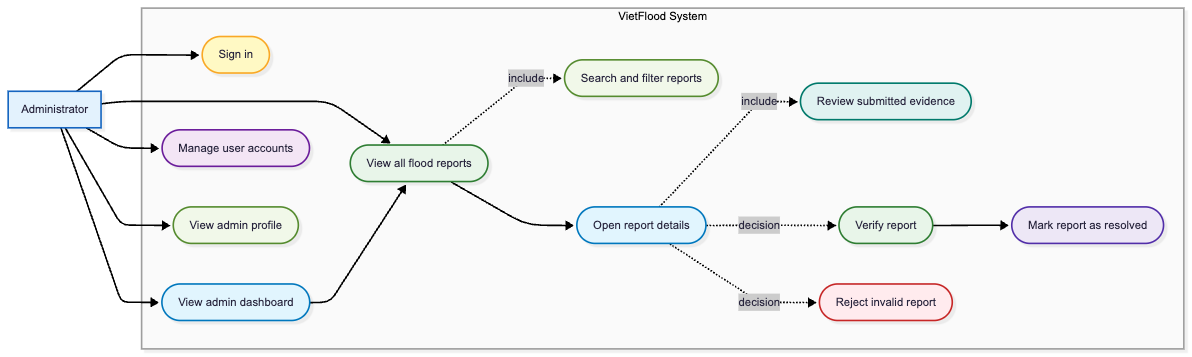
\includegraphics[width=0.74\linewidth,height=0.36\textheight,keepaspectratio]{images/figure3-3-admin-use-case.png}
    \caption{Use case diagram for the administrator actor in VietFlood.}
    \label{fig:method-admin-usecase}
\end{figure}

\section{Materials and Development Tools}

VietFlood was developed from four source-code modules. The backend module contains the NestJS API gateway and microservices \cite{nestjsDocs,nestjsMicroservicesDocs}. The shared module contains reusable logging, Redis, and Cloudinary utilities. The mobile module contains the Expo React Native application \cite{expoDocs,reactNativeDocs}. The web module contains the Next.js administrator dashboard \cite{nextjsDocs}. The main tools are summarized in Table~\ref{tab:method-tools}.

\begin{table}[htbp]
\centering
\caption{Main materials and tools used in VietFlood development.}
\label{tab:method-tools}
\begin{tabular}{|>{\raggedright\arraybackslash}p{4cm}|>{\raggedright\arraybackslash}p{9cm}|}
\hline
\textbf{Area} & \textbf{Tools and purpose} \\
\hline
Backend & NestJS, TypeScript, TypeORM, PostgreSQL, RabbitMQ, Redis, Socket.IO, JWT, bcrypt. \\
\hline
Shared package & \texttt{vietflood\_common} for structured logging, Redis client setup, and Cloudinary file operations. \\
\hline
Mobile client & Expo, React Native, TypeScript, React Navigation, Redux Toolkit, image picking, secure token storage, device location, and Vietnam Provinces Open API. \\
\hline
Web dashboard & Next.js, React, TypeScript, Tailwind CSS, protected admin login, token refresh, report overview, search, filtering, evidence preview, and status update. \\
\hline
Runtime infrastructure & Docker, Docker Compose, PostgreSQL, Redis, RabbitMQ, Cloudinary, and Azure App Service configuration. \\
\hline
\end{tabular}
\end{table}

\section{System Design Method}

The backend was designed as a small microservice system. The service split was kept limited because too many services would make the prototype harder to operate without adding much value. Microservice literature emphasizes that service boundaries should clarify responsibility and support change, while still accounting for operational cost \cite{fowlerLewis2014microservices,dragoni2017microservices,thones2015microservices}. VietFlood therefore uses only the boundaries needed for the thesis: public access, authentication, report management, shared infrastructure utilities, and supporting infrastructure.

The API gateway receives HTTP and WebSocket traffic from clients. The authentication service owns registration, sign-in, refresh tokens, profile loading, logout, admin seeding, and user management. The reports service owns report creation, report lookup, evidence metadata, status changes, cache updates, and report deletion. Redis supports cached report lookup, RabbitMQ carries service messages, PostgreSQL stores persistent data, and Cloudinary stores uploaded images.

\begin{figure}[htbp]
    \centering
    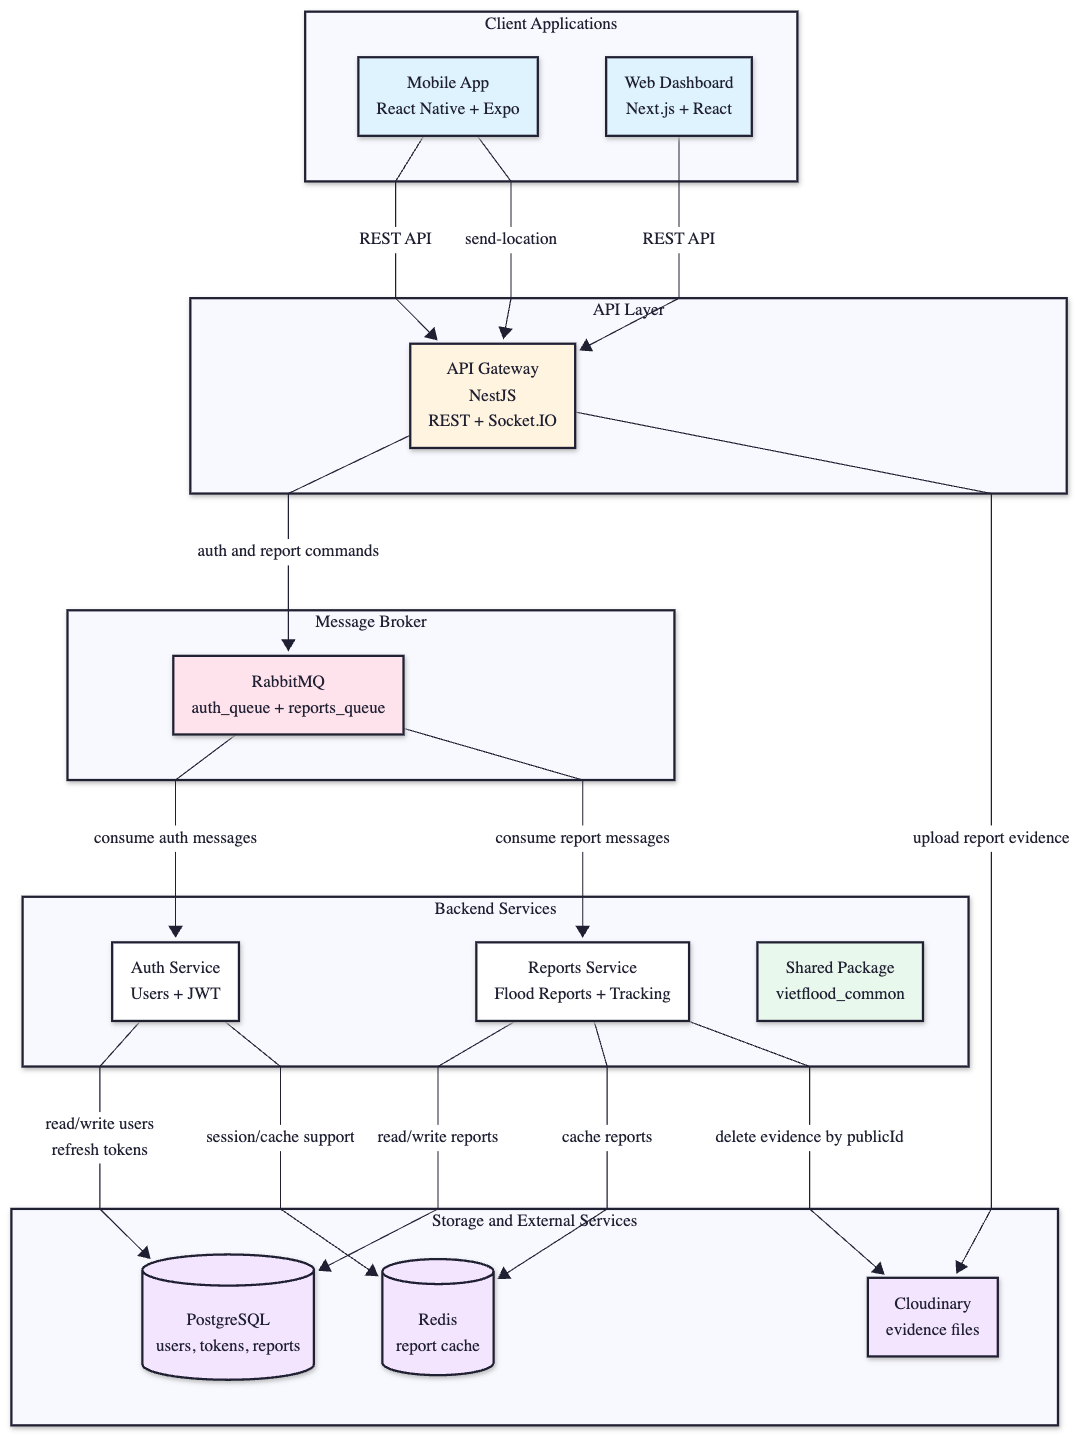
\includegraphics[width=1\linewidth,height=0.44\textheight,keepaspectratio]{images/figure3-4-system-architecture.png}
    \caption{VietFlood system architecture diagram.}
    \label{fig:method-system-architecture}
\end{figure}

\subsection{API Gateway Method}

The gateway exposes the routes used by both client applications. Authentication routes are grouped under \texttt{/auth}, and report routes are grouped under \texttt{/reports}. Report creation uses multipart upload through the \texttt{files} field. The gateway holds uploaded files in memory long enough to upload them to Cloudinary. It then forwards the report data and evidence metadata to the reports service.

The gateway also applies authentication and role checks. Citizen routes are used for personal report operations. Broader report-reading routes are available to relief and admin users. Admin-specific operations are protected separately. This method keeps the clients simple while still enforcing access rules on the backend.

\subsection{Message Communication Method}

RabbitMQ is used for communication between the gateway and internal services \cite{rabbitmqConfirmsDocs}. Authentication messages are consumed by the auth service, while report messages are consumed by the reports service. The authentication service handles message patterns for registration, sign-in, profile loading, token refresh, logout, and user operations. The reports service handles report creation, listing, lookup, update, and deletion.

This message-based method makes boundaries visible during development. A failed report submission can be inspected at the gateway request, the Cloudinary upload step, the RabbitMQ message, or the reports service handler. The gateway also uses controlled service-call behavior so a slow internal service does not leave the client waiting without a response.

\section{Database Design Method}

The database design was derived from the report workflow. A report needs a user owner, location fields, status, urgency, severity, evidence metadata, and timestamps. The backend uses PostgreSQL as the main database and TypeORM entities to map application objects to database tables \cite{typeormDocs,postgresqlJsonDocs}.

The user entity stores email, username, phone, hashed password, role, name fields, date of birth, address line, ward, province, and timestamps. Email, username, and phone are unique. The supported roles are \texttt{citizen}, \texttt{relief}, and \texttt{admin}.

The report entity stores category arrays, description, image URLs, evidence JSON, province, ward, address line, latitude, longitude, status, reporter name, urgency, severity, timestamps, and owner user ID. Evidence is stored as JSON metadata because each uploaded item needs a URL, Cloudinary public ID, and resource type. PostgreSQL supports this kind of flexible structured field through JSON storage \cite{postgresqlJsonDocs}.

\begin{figure}[htbp]
    \centering
    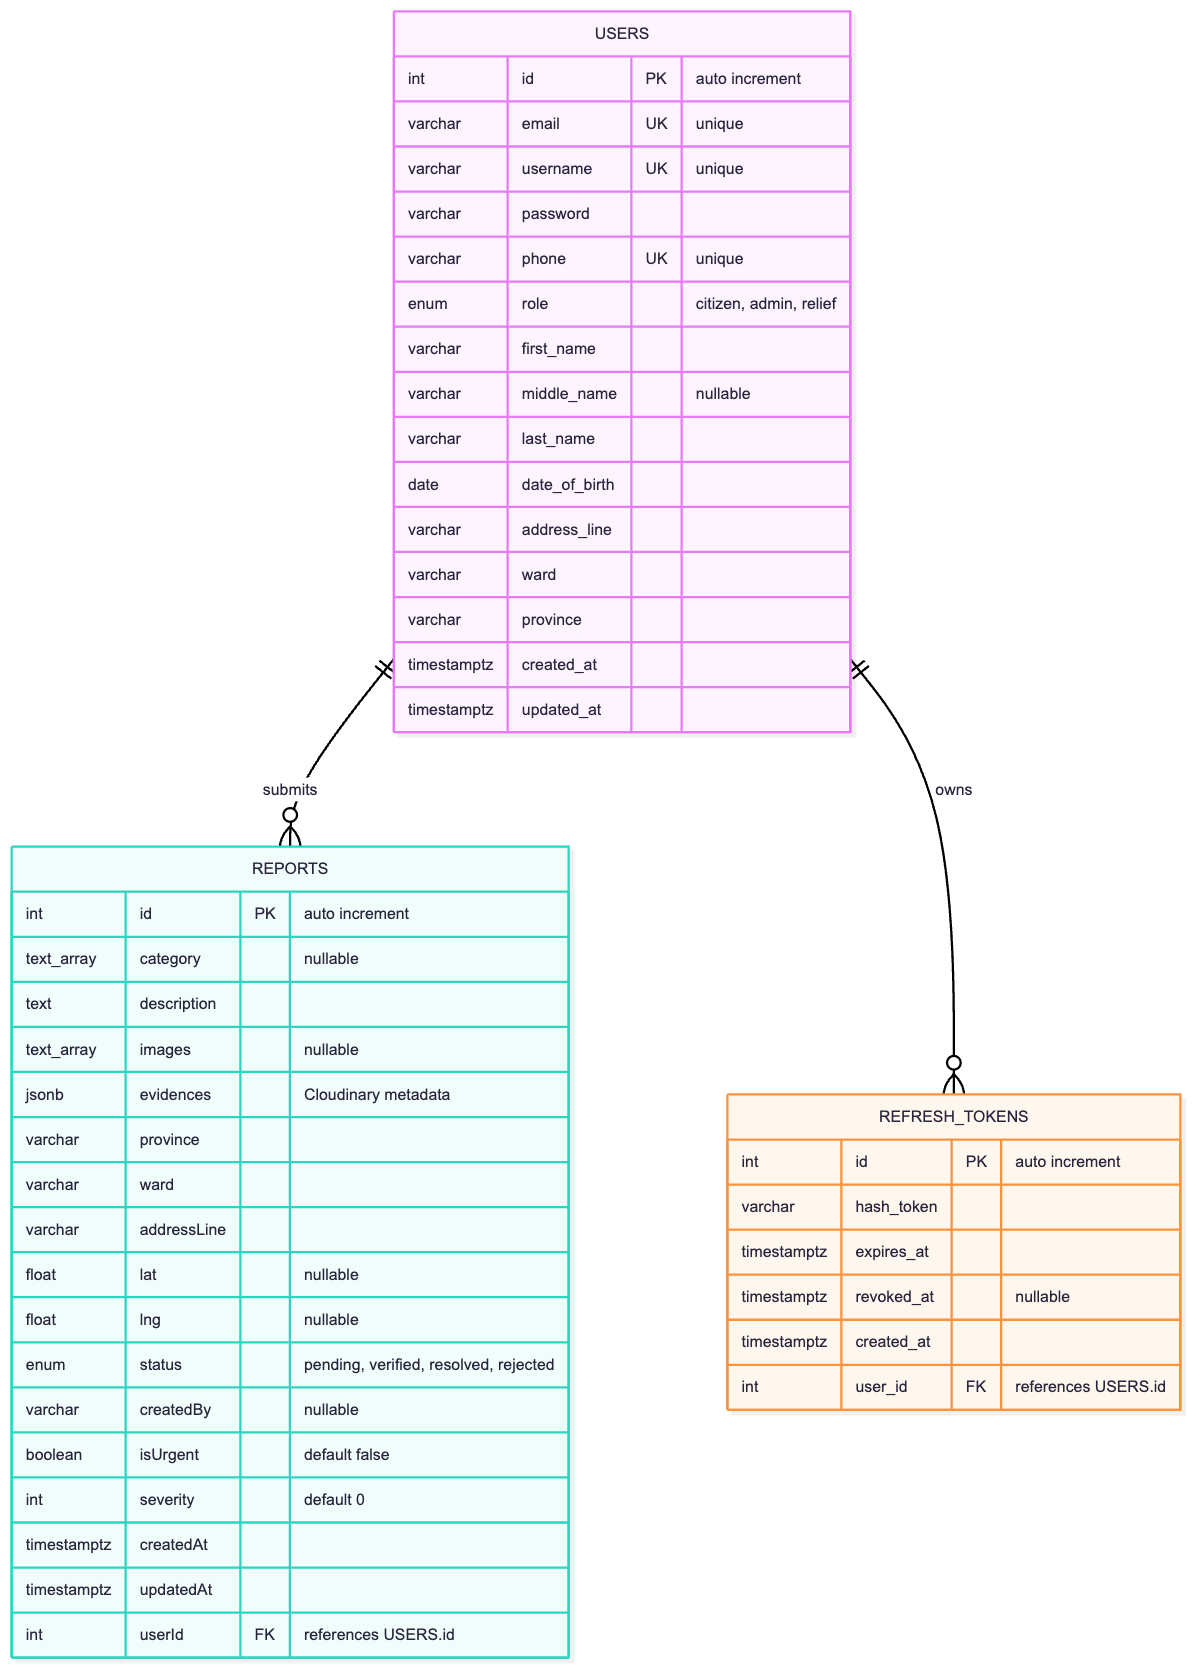
\includegraphics[width=0.9\linewidth,height=0.42\textheight,keepaspectratio]{images/figure3-5-database-schema.png}
    \caption{Database schema diagram for VietFlood.}
    \label{fig:method-database-schema}
\end{figure}

\subsection{Cache Method}

Redis is used as a cache and not as the source of truth \cite{redisDocs}. When a report is created, the reports service stores a cached copy using a key pattern based on the report ID. When a report is requested, the service can check Redis before reading from PostgreSQL. When the report is updated or deleted, the cache entry is refreshed or removed.

The cache scope is intentionally narrow. Report ownership, status, evidence, and location remain in PostgreSQL. Redis only provides a temporary lookup copy. This keeps invalidation understandable for the prototype.

\section{Workflow Design Method}

The main workflow is citizen report creation. The citizen fills in category, description, administrative location, coordinates, urgency, severity, and optional image evidence. The mobile app sends the report as a multipart request. The API gateway authenticates the user, uploads evidence files to Cloudinary, and forwards the completed payload to the reports service through RabbitMQ. The reports service saves the report in PostgreSQL and creates or updates the Redis cache entry.

\begin{figure}[htbp]
    \centering
    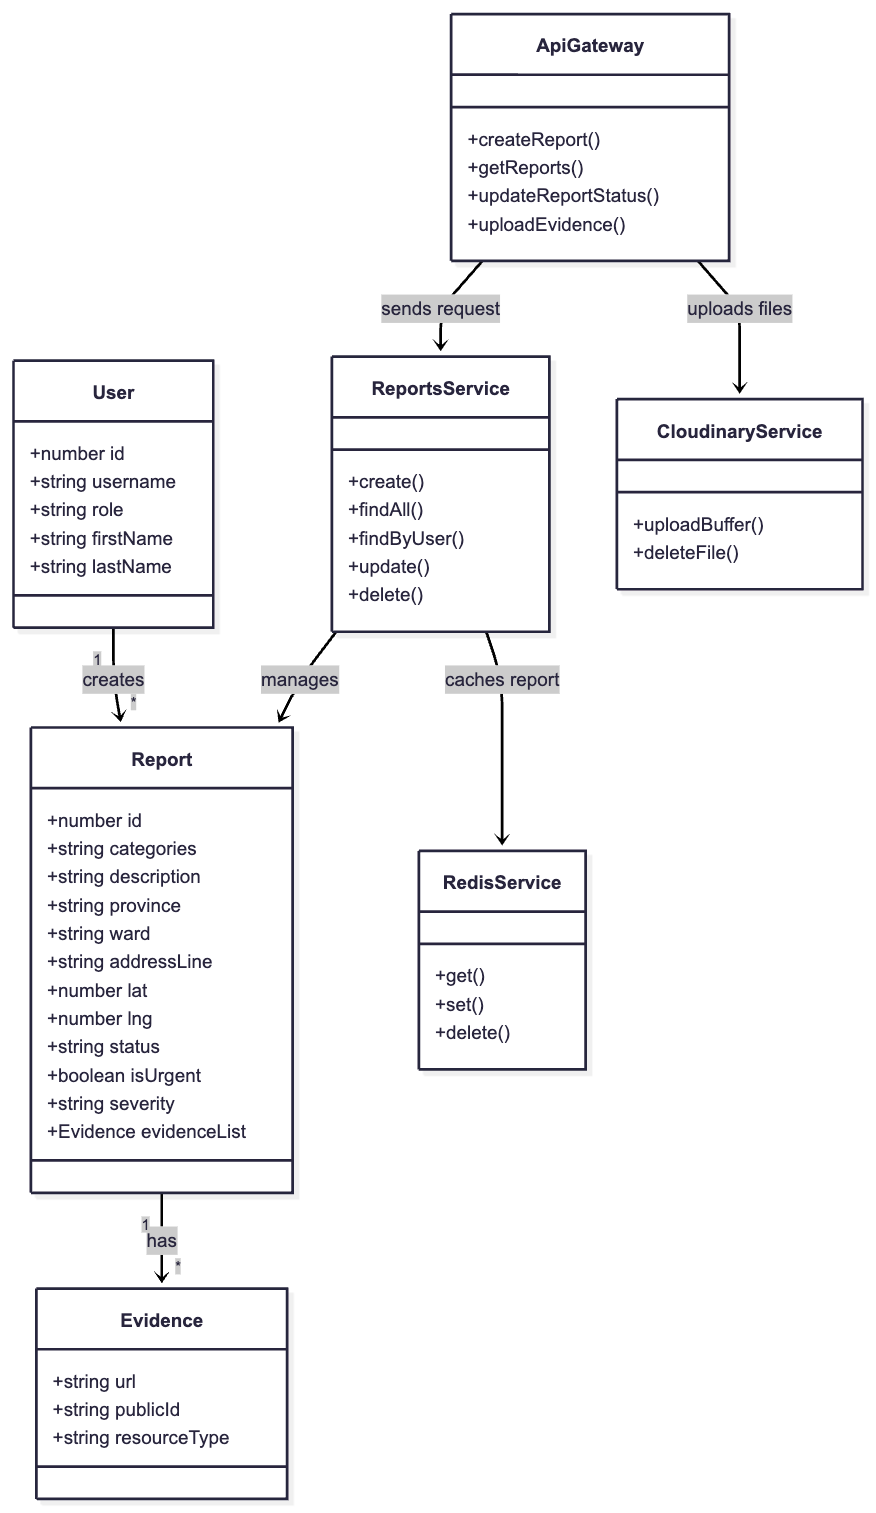
\includegraphics[width=0.9\linewidth,height=0.42\textheight,keepaspectratio]{images/figure3-6-report-class-diagram.png}
    \caption{Class or module diagram for the report workflow.}
    \label{fig:method-report-class}
\end{figure}

\begin{figure}[htbp]
    \centering
    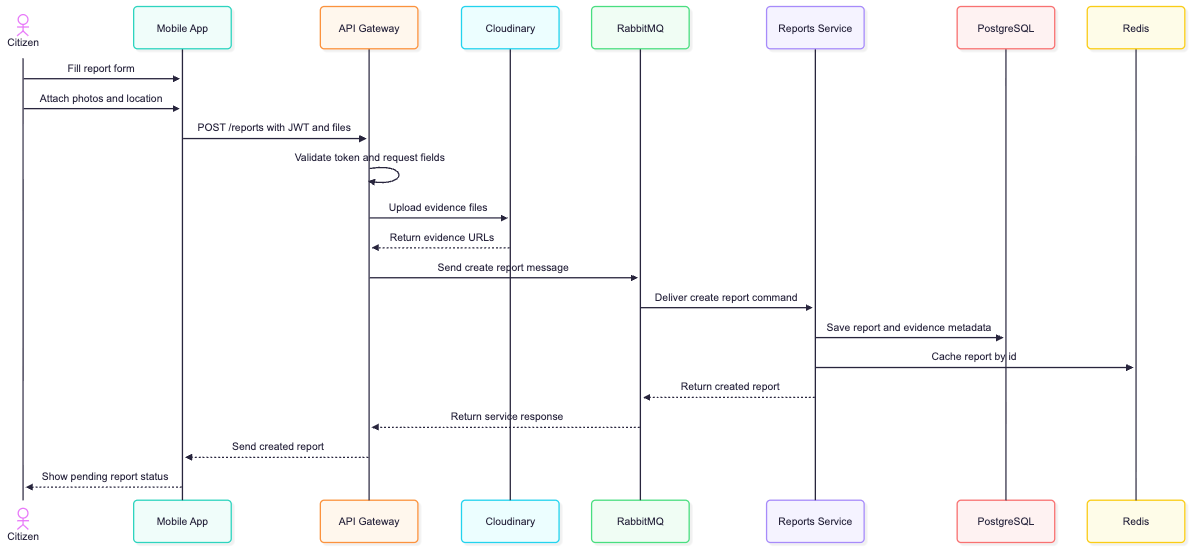
\includegraphics[width=0.9\linewidth,height=0.44\textheight,keepaspectratio]{images/figure3-7-create-report-sequence.png}
    \caption{Sequence diagram for creating a VietFlood report.}
    \label{fig:method-create-report-sequence}
\end{figure}

\subsection{Evidence Handling Method}

Evidence images are not stored in PostgreSQL as raw files. The gateway uploads image buffers to Cloudinary under the report folder \cite{cloudinaryUploadDocs}. The reports service stores the returned URL, public ID, and resource type with the report. The URL is used by the mobile app and dashboard for display. The public ID is kept so related media can be removed when a report is deleted.

This method keeps the database focused on structured data while Cloudinary handles media storage and delivery. It also means media credentials must be provided through environment configuration instead of being written into the source code.

\subsection{Status Review Method}

Status review is handled as an administrator workflow. Relief users can read broader report information and use map-related screens, but verification and rejection are not part of the relief role in this thesis. The administrator dashboard sends status updates through the gateway. The reports service checks the existing report, merges new evidence metadata when needed, updates the status, and refreshes the cache entry.

\section{Client Application Method}

\subsection{Mobile Application Method}

The mobile app was developed with Expo React Native and TypeScript \cite{expoDocs,reactNativeDocs,typescriptDocs}. It supports token-based authentication, profile screens, report creation, report lists, relief report details, map screens, settings, localization, and role-aware navigation. Redux Toolkit supports application state around authentication and client-side data flow \cite{reduxToolkitDocs}.

The mobile report service normalizes backend data before rendering it. This is needed because report fields may appear in different naming styles, such as snake case and camel case, or as \texttt{lat}/\texttt{lng} and \texttt{latitude}/\texttt{longitude}. The mobile location method also combines administrative division data from the Vietnam Provinces Open API with device location when permission is available \cite{vietnamProvincesOpenApi}.

\subsection{Web Dashboard Method}

The web dashboard was developed with Next.js, React, TypeScript, and Tailwind CSS \cite{nextjsDocs,reactDocs,typescriptDocs,tailwindDocs}. It is focused on administrator review. The dashboard signs in through the backend, stores access and refresh tokens, refreshes sessions when needed, loads the current profile, and blocks non-admin users from the admin workspace.

After authentication, the dashboard loads report data from the gateway and displays report cards with status, category, severity, address, description, reporter information, and evidence thumbnails. It also provides search, filtering, user management, and status update controls.

\section{Real-Time Tracking Method}

The backend includes a Socket.IO gateway for live location updates \cite{socketioDocs}. A connected client can emit a location event with latitude, longitude, accuracy, heading, speed, and timestamp. The gateway checks latitude and longitude ranges before broadcasting the accepted location to other clients. Invalid payloads receive an error event. When a socket disconnects, the gateway announces the disconnected client.

This feature is treated as a prototype path. It proves that the backend can receive and broadcast live location data. Future work would still be needed for authenticated socket sessions, route assignment, persistent location history, and operational use in real relief coordination.

\section{Validation Method}

Validation was performed through source-level checks and workflow checks. Source-level checks focused on whether each module matched its responsibility: the gateway handled client-facing access, the authentication service handled identity and tokens, the reports service handled report data, and the shared package handled reusable infrastructure. Docker Compose was used as the repeatable local environment for backend services and infrastructure dependencies \cite{dockerComposeDocs}.

Workflow checks focused on the main paths of the prototype:

\begin{itemize}
    \item citizen registration, sign-in, and profile loading;
    \item citizen report creation with category, address, coordinates, urgency, severity, and images;
    \item evidence upload to Cloudinary and metadata storage in PostgreSQL;
    \item report list loading for citizen, relief, and admin views;
    \item administrator report status update through the web dashboard;
    \item Redis cache creation, refresh, and deletion during report changes;
    \item Docker Compose startup for backend services, Redis, and RabbitMQ.
\end{itemize}

This validation method matches the current stage of VietFlood. The system is a working prototype, not a certified emergency-response platform. The checks therefore focus on whether the main reporting, evidence, review, cache, and service-integration flows operate according to the design.
